% The equation of a plane $P$ passing through the line of intersection of the planes $P_{1}$ and $P_{2}$ has the form,
% \begin{align}
%    P : P_{1} + \lambda P_{2}\label{sep/2/28eq1}
% \end{align}
% %
% General equation of plane is given by
% \begin{align}
%     \vec{n}^T\vec{x}=c
% \end{align}
% Where $\vec{n}$ is normal vector to the plane
\begin{lemma}
   The equation of a plane passing through intersection of planes
   \begin{align}
    \vec{n_{1}}^T\vec{x}&=c_{1}\\ \vec{n_{2}}^T\vec{x}&=c_{2}
   \end{align}
   and perpendicular to plane
   \begin{align}
     \vec{n_{3}}^T\vec{x}&=c_{3}
   \end{align}
   is given by 
   \begin{align}
      \vec{n_{4}}^T\vec{x}&=c_{4}
   \end{align}
   where 
   \begin{align}
       \vec{n_{4}} = \vec{n_{1}} - \brak{\frac{\vec{n_{3}^T\vec{n_1}}}{\vec{n_{3}^T\vec{n_2}}}}\vec{n_2}\\
       c_{4} = c_{1} - \brak{\frac{\vec{n_{3}^T\vec{n_1}}}{\vec{n_{3}^T\vec{n_2}}}}c_{2}
   \end{align}
\end{lemma}
\begin{proof}
   Let $P$ be the plane that passes through intersection 2 given planes.\\  From \eqref{sep/2/28/eq1}, equation of $P$ has the form,
   \begin{align}
       \vec{n_{1}}^T\vec{x} + \lambda\brak{\vec{n_{2}}^T\vec{x}} = c_{1} + \lambda\brak{c_{2}}\\
       \implies \brak{\vec{n_{1}}+\lambda\vec{n_{2}}}^T\vec{x} = c_{1} + \lambda\brak{c_{2}}
   \end{align}
  Normal vector to plane $P$ is,
 \begin{align}
     \vec{n_{4}} = \vec{n_{1}}+\lambda\vec{n_{2}}
 \end{align}
 As $P$ is perpendicular to the third plane i.e. angle between normal vectors is $90\degree$, 
 \begin{align}
     &\cos\brak{90\degree} = 0 = \dfrac{\vec{n_{3}}^T\vec{n_{4}}}{\norm{\vec{n_{3}}}\norm{\vec{n_{4}}}}\\
    \implies &\vec{n_{3}}^T\vec{n_{4}} = 0\\
    \implies &\vec{n_{3}}^T\brak{\vec{n_{1}}+\lambda\vec{n_{2}}} = 0\\
    \implies &\lambda = \frac{-\vec{n_{3}^T\vec{n_1}}}{\vec{n_{3}^T\vec{n_2}}}
 \end{align}
 Therefore equation of plane $P$ is,
 \begin{align}
     \brak{\vec{n_{1}} - \brak{\frac{\vec{n_{3}^T\vec{n_1}}}{\vec{n_{3}^T\vec{n_2}}}}\vec{n_2}}^T\vec{x} = c_{1} - \brak{\frac{\vec{n_{3}^T\vec{n_1}}}{\vec{n_{3}^T\vec{n_2}}}}c_{2}
 \end{align}
\end{proof}
For the given problem,
\begin{align}
  \vec{n_{1}}=\myvec{1\\1\\1}\\c_{1}=1,
  \vec{n_{2}}=\myvec{2\\3\\4},
     c_{2}=5\\
  \vec{n_{3}}=\myvec{1\\-1\\1}\\c_{3}=0 
 \end{align}
Solving the above we get,
\begin{align}
    \lambda = \frac{-1}{3},
    \vec{n_{4}} = \myvec{\frac{1}{3}\\0\\\frac{-1}{3}},
    c_{4} = \frac{-2}{3}
\end{align}
We have equation of the plane as,
\begin{align}
    \myvec{\frac{1}{3}&0&\frac{-1}{3}}\vec{x} = \frac{-2}{3} 
\end{align}
\begin{figure}[!ht]
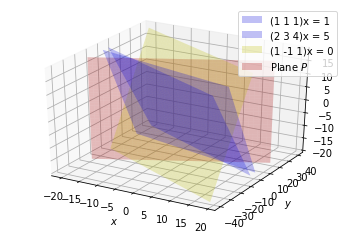
\includegraphics[ width=\columnwidth]{solutions/sep/2/28/figures/planes.png}
\caption{Plane $P$ passing through intersection of $P_{1}$ and $P_{2}$ and perpendicular to $P_{3}$}
\label{sep/2/28fig:Line }	
\end{figure}
